\def\QRCODE{TB_image_TUT.IMG.image_segmentation_follicule_pythonqrcode.png}
\def\QRPAGE{http://www.iptutorials.science/tree/master/TB_image/TUT.IMG.image_segmentation_follicule/python}
\pcorrectionsection{Python correction}

\begin{python}
import numpy as np
import matplotlib.pyplot as plt
from scipy import misc,ndimage
from skimage import morphology
\end{python}

\vspace*{-.8\baselineskip}

\subsection{Vascularization}\vspace*{-3pt}
\subsubsection{Antrum segmentation}
The first step consists in the segmentation of the antrum by thresholding the blue component. Some post-processes are used to remove artifacts such as holes. This is illustrated in Fig. \ref{fig:segfollicle:python:vascularization}.


\begin{python}
A = imageio.imread('follicle.png');
plt.imshow(A);
plt.show();
## Antrum
# segmentation by mathematical morphology
# manual selection of the antrum
B = A[:,:,2];
antrum = B > 220;
L = morphology.label(antrum, connectivity=2);
antrum = L == L[300,300];
antrum = ndimage.morphology.binary_fill_holes(antrum);
plt.imshow(antrum);
plt.title('Antrum')
plt.show();
\end{python}

\subsubsection{Theca segmentation}
The second step provides the segmentation of the theca which is extracted as a spatial region (corona) adjacent to and outside the antrum. The width of the corona is selected by the user (expert).
\begin{python}
se40 = morphology.disk(40);
theca = morphology.binary_dilation(antrum, selem = se40);
theca = theca - antrum;
plt.imshow(theca); plt.title('Theca')
plt.show()
\end{python}

\subsubsection{Vascularization segmentation}
The final step extracts the vascularization of the considered follicle. Pixels belonging to the vascularization are considered to have a low blue component and they should also be included in the antrum of the follicle.
\begin{python}
vascularization = B < 140;
vascularization = vascularization * theca;
plt.imshow(vascularization);
plt.title('vascularization')
plt.show();
\end{python}

\subsubsection{Results}
\begin{figure}[H]
\centering\caption{Extraction of the different components of the follicle.}%
 \subfloat[Original image.]{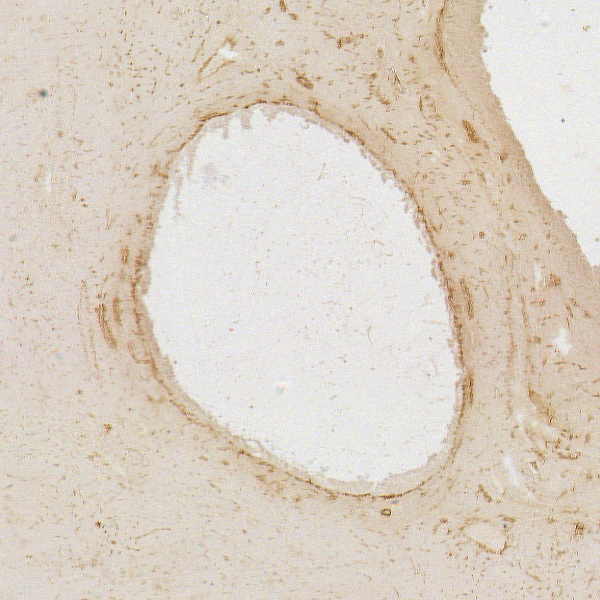
\includegraphics[width=4cm]{follicle.png}}
 
 \subfloat[Antrum.]{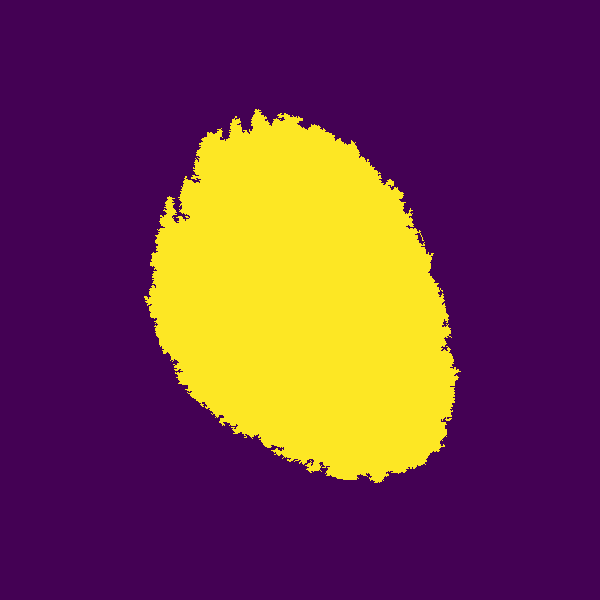
\includegraphics[width=.3\linewidth]{antrum.png}}\hfill
 \subfloat[Theca.]{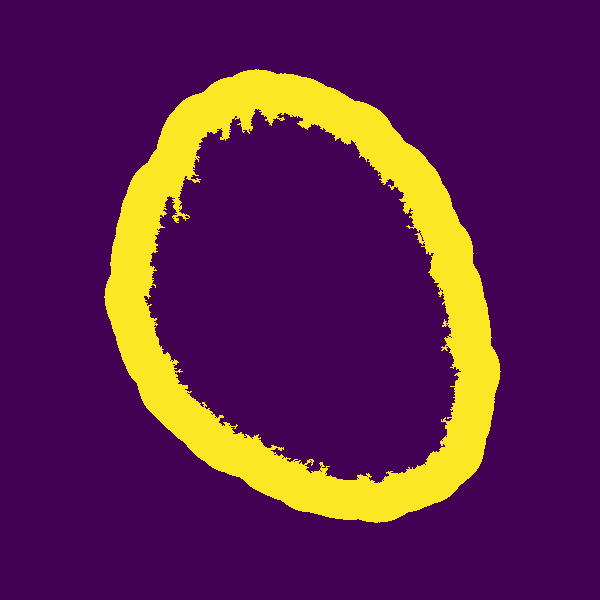
\includegraphics[width=.3\linewidth]{theca.png}}\hfill
 \subfloat[Vascularization.]{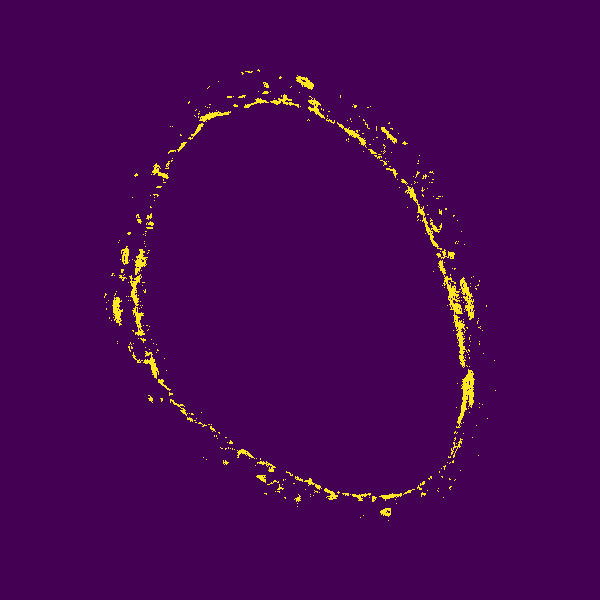
\includegraphics[width=.3\linewidth]{vascularization.png}}%
 \label{fig:segfollicle:python:vascularization}%
\end{figure}

\subsection{Granulosa cells}
\subsubsection{First solution}
The granulosa cells have a low contrast, so it is difficlut to use thresholding techniques. But we know they are localized between the antrum and the vascularization. Nevertheless the vascularization is not a closed region outside the antrum. Therefore, the proposed solution consits in firt trying to close the vascularization region and taking the corona between this region and the antrum. The result is shown in Fig. \ref{fig:segfollicle:python:granulosa}.

\begin{python}
se10 = morphology.disk(10);
dil = 1-morphology.binary_closing(vascularization, se10);
L = morphology.label(dil, connectivity=1);
dil = L == L[300,300];
granulosa = dil - antrum;
plt.imshow(granulosa);
plt.title('granulosa')
plt.show()
\end{python}

\begin{figure}[htbp]
\centering\caption{Extraction of the granulosa cells of the follicle.}%
 \subfloat[Original image.]{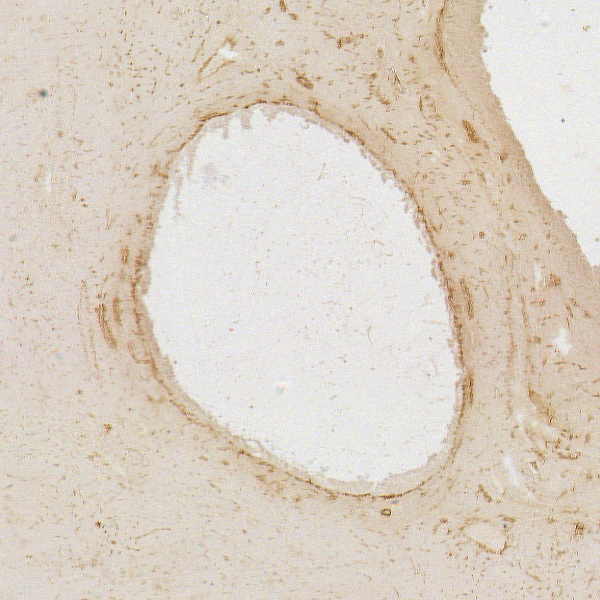
\includegraphics[width=.3\linewidth]{follicle.png}}\hfill
 \subfloat[Granulosa cells.]{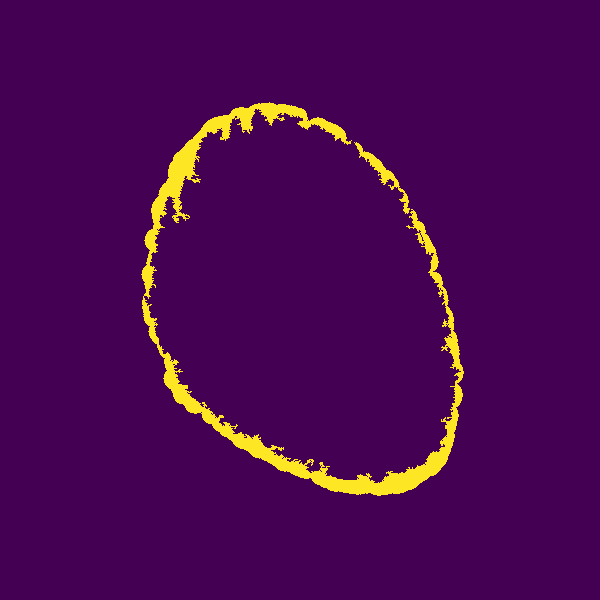
\includegraphics[width=.3\linewidth]{granulosa.png}}\hfill
 \subfloat[Segmentation of the different parts.]{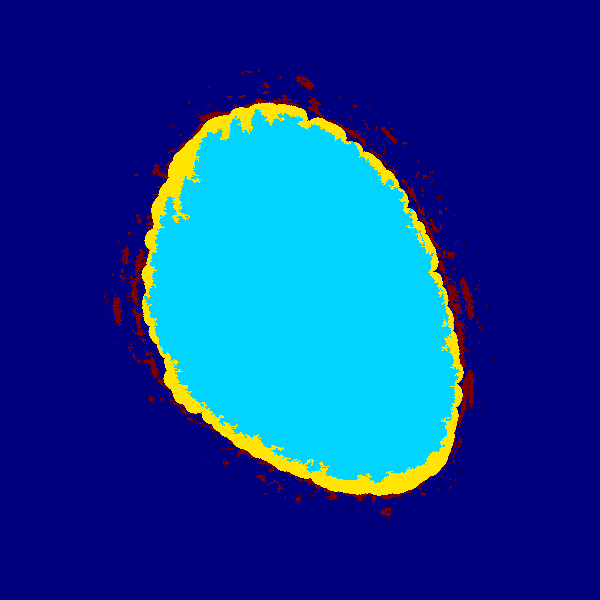
\includegraphics[width=.3\linewidth]{result_python.png}}%
 \label{fig:segfollicle:python:granulosa}%
\end{figure}

\subsubsection{Second solution}
This first solution is not really robust. The closing of the vascularization region is not really accurate. A more robust solution consists in using deformable models to get the corona between the vascularization and the antrum. But this kind of method is out of the scope of this tutorial.

\subsection{Quantification}
The quantification is easy to process. In addition, we can represent the different extracted components of the follicle in false colors.

\begin{python}
result = antrum + 2*granulosa + 3*vascularization;
plt.imshow(result, cmap='jet');
plt.show();
plt.imsave("result.png", result, cmap='jet');

follicle = antrum + theca;
q_vascularization = np.sum(vascularization) / np.sum(follicle);
print('vascularization: ', q_vascularization)
q_granulosa = np.sum(granulosa)/np.sum(follicle);
print('Granulosa: ', q_granulosa);
\end{python}

\noindent This quantification gives:
\begin{sh}
vascularization:  0.0428495233516
Granulosa:  0.0913707490403
\end{sh}